\documentclass[a4paper,11pt,UTF8]{article}
\usepackage{ctex}
\usepackage{amsmath,amsthm,amssymb,amsfonts}
\usepackage{amsmath}
\usepackage[a4paper]{geometry}
\usepackage{graphicx}
\usepackage{microtype}
\usepackage{siunitx}
\usepackage{booktabs}
\usepackage[colorlinks=false, pdfborder={0 0 0}]{hyperref}
\usepackage{cleveref}
\usepackage{esint} 
\usepackage{graphicx}
\usepackage{ragged2e}
\usepackage{pifont}
\usepackage{extarrows}
\usepackage{mathptmx}
\usepackage{float}
\usepackage{caption}
\captionsetup[figure]{name={Figure}}
%opening
\title{Microelectronics Circuit Analysis and Design Homework(6th)}
\author{Yuejin Xie \quad U202210333}
\date{Sept 27th, 2023}
\begin{document}
\maketitle
\noindent4.15 For the NMOS common-source amplifier in Figure P4.15, the transistor
parameters are: $V_{T N }= 0.8$V, $K_n = 1\text{mA/V}^2$, and $\lambda = 0$. The circuit parameters
are $V_{DD} = 5 $V, $R_S = 1 k\Omega$, $R_D = 4 k\Omega$, $R_1 = 225 k\Omega$, and
$R_2 = 175 k\Omega$. (a) Calculate the quiescent values $I_{DQ}$ and $V_{DSQ}$. (b) Determine
the small-signal voltage gain for $R_L =\infty$. (c) Determine the value of
$R_L$ that will reduce the small-signal voltage gain to 75 percent of the value
found in part (b).\\
\begin{figure}[H] 
	\centering 
	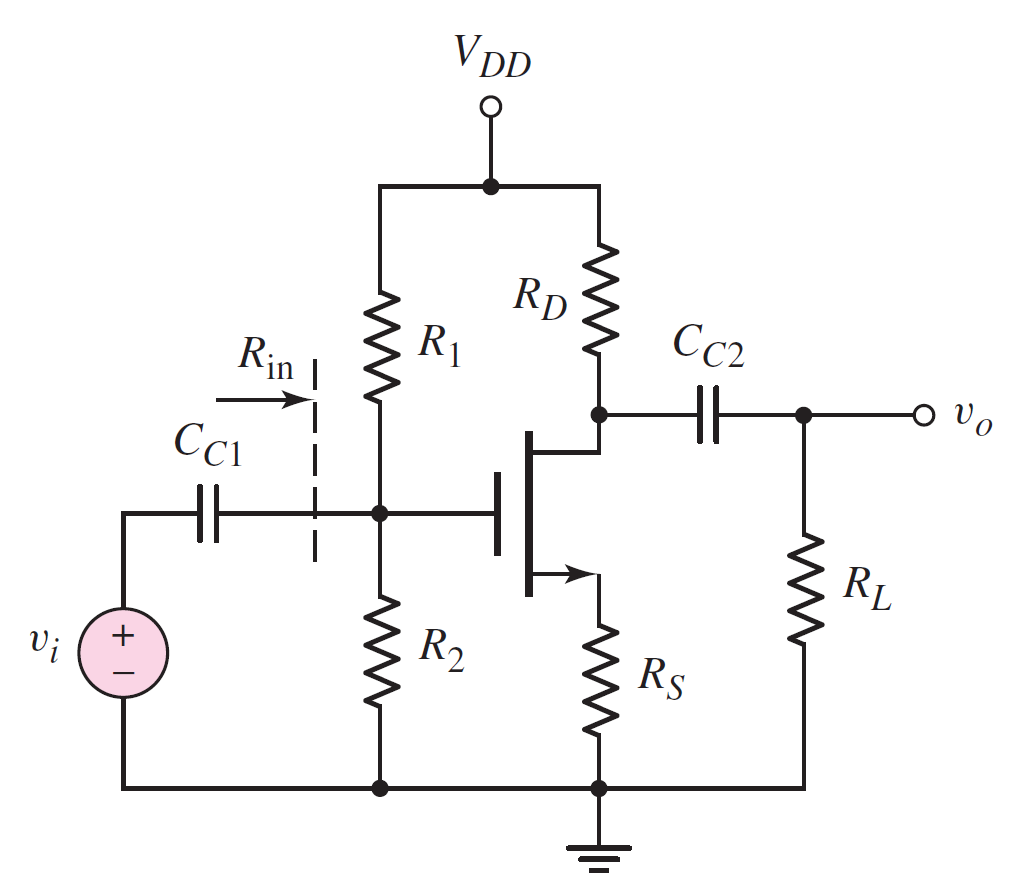
\includegraphics[scale=0.3]{MD4.15.png}
	\caption{Problem 4.15/4.17}
\end{figure}
\noindent4.17 Repeat Problem 4.15 if the source resistor is bypassed by a source capacitor
$C_S$.\\
D4.26 Design the common-source circuit in Figure P4.26 using an n-channel
MOSFET with $\lambda = 0$. The quiescent values are to be $I_{DQ} = 6 $mA,
$V_{GSQ} = 2.8$ V, and $V_{DSQ} = $10 V. The transconductance is $g_m = 2.2 $mA/V.
Let $R_L = 1 k\Omega$, $A_v = -1$, and $R_{in} = 100 k\Omega$. Find $R_1, R_2, R_S, R_D, K_n$, and $V_{T N}$ .\\
\begin{figure}[H] 
	\centering 
	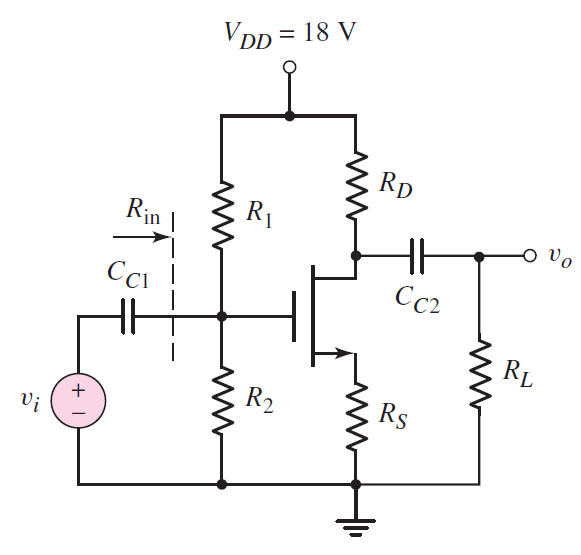
\includegraphics[scale=0.5]{MD4.26.png}
	\caption{Problem 4.26}
\end{figure}
\end{document}